\documentclass[12pt]{article}
\usepackage[margin=1in]{geometry}
\usepackage{multirow}
\usepackage{cmap}
\usepackage[T2A]{fontenc}
\usepackage{float}
\usepackage[utf8]{inputenc}
\usepackage{mathtext}

\usepackage[english]{babel}
\usepackage{commath}
\usepackage{gensymb}
\usepackage{caption, subcaption}
\usepackage{amsfonts}
\usepackage{amssymb}
\usepackage{amsmath}
\usepackage{amsthm}
\usepackage{mathtools}
\usepackage{xcolor}
% \usepackage{indentfirst}
\usepackage{parskip}
\usepackage{hyperref}
\usepackage{url}
\usepackage{titlesec}
\titleformat{\subsubsection}[runin]
        {\normalfont\bfseries}
        {\thesubsection}
        {0.5em}
        {}
        [.]

% \usepackage{fancyhdr}
 
% \pagestyle{fancy}
% \fancyhf{}
% \rhead{Mikhail Terekhov}
% \lhead{Research Interests}
% \cfoot{\thepage}

\newcommand{\R}{\mathbb{R}}
\newcommand{\E}{\mathbb{E}}
\newcommand{\PP}{\mathbb{P}}
\DeclareMathOperator*{\argmin}{arg\,min}
\DeclareMathOperator*{\argmax}{arg\,max}

\newcommand{\todo}[1]{{\color{red} #1}}

\newtheorem{theorem}{Theorem}
\newtheorem{lemma}{Lemma}
\newtheorem{assumption}{Assumption}


\newtheorem*{assumptionp}{Assumption 1'}



\begin{document}

\begin{center}
  {\LARGE \bf{Are important features more interpretable?}}
\end{center}
\vspace{-1em}

\noindent\rule{\textwidth}{1pt}

  
\begin{center}
  {\large \bf{Mikhail Terekhov}} \\
  % \vspace{0.5em}
  Final project for the AGISF course
\end{center}

% \begin{itemize}
  % \item The key idea: connecting "importance" and "interpretability"
  % \item Related work
    % \begin{itemize}
      % \item Link to sparsified nets work by Tegmark
      % \item Tegmark also defines "importance" crudely by the sum of abs. values of incoming and outgoing weights
      % \item If most neurons are not interpretable, but a few that are also happen to be important, interpretability research is more relevant.
    % \end{itemize}
  % \item Work overview: Microscope down, Lucid struggles with TF2, partial\_run breakthrough, filling the form myself.
  % \item Importance measure
  % \item Interpretability formular
  % \item Results: overall distr of importance, scatter \& hist plots.
    % \begin{itemize}
      % \item Discuss checking method: substitute the known activations
      % \item Checking my activation examples vs the known values in the appendix of the interp paper
      % \item Can discuss whether intermediate outputs in InceptionV1 made neurons more interpretable, maybe link to the "preferred basis" idea from the superposition interpretability blog posts
    % \end{itemize}
  % \item Future work: making it proper would require more effort. Automated "recognizability", use Max's suggestions; fancier importance measures, working with bigger models.
    % \begin{itemize}
      % \item Maybe in big networks there is no interpretable neurons at all!
      % \item InceptionV1: 1000 classes vs 830 features: the need for superposition is not so high
      % \item Used limited data even compared to the microscope: sometimes the data reveals that negative activations are the important thing
      % \item proper evaluation requires more input images, more compute, automated interpretability testing
      % \item Make it into a more general story: interpretability as qualitative analysis of individual components vs quantitative interventions; these two approaches could be connected.  
% \end{itemize}
\section{Introduction}
The idea for this project was born out of Stephen Casper's ``Engineer's Interpretability Sequence''. In part VI~\cite{cas2023interpretability}, he critisizes current mechanistic interpretability approaches along several directions. One of his arguments is that feature visualizations in the papers are often cherry-picked, while features ``in the wild'' are more often non-interpretable. This claim can be considered in conjunction with the end goal of mechanistic interpretability, which is to extract an algorithm that underlies the neural network's predictive power. 
A prominent approach to constructing such algorithms is through \emph{circuits}~\cite{olah2020zoom}. A circuit is a subgraph of the initial neural net that connects individual features in different layers in meaningful ways, composing complicated abstractions in later layers out of simpler ones in earlier layers. Authors of~\cite{olah2020zoom} use an example of a ``car detector'' being composed of a ``window detector'', ``car body detector'', and a ``wheel detector''. Crucially, the components of this circuit are all somewhat recognizable in the individual feature visualizations. Features in convolutional neural nets (CNNs) can be visualized using approaches from~\cite{olah2017feature}. These approaches include maximizing the activation over the input image with some regularization and looking for images from the dataset that activate the feature the most. Strong negative activations can be considered as well. If the feature visualizations do not make sense to a human observer, then the feature cannot be manually put into a circuit, and the critique of~\cite{cas2023interpretability} applies. Thus, if most features are not interpretable, circuits can only explain a minority of the network's inner workings.

In this project, I consider an alternative hypothesis:

\noindent\fbox{%
    \parbox{\textwidth}{%
      \textit{Are the most important features for network's performance more interpretable?}
    }%
}

If this hypothesis holds, mechanistic interpretability research is more promising: even though the majority of features are not interpretable, they can be discarded without significant performance degradation. Otherwise, we have less hope: interpretable features are a minor artifact and the network is still mostly opaque. 

Some evidence for the possibility of this hypothesis is provided by the success of \emph{sparsification} of neural networks. As it turns out, the majority of features can indeed be pruned from a CNN without a performance drop~\cite{anwar2017structured}. This still leaves open the question of whether the remaining features are the interpretable ones. Sparsity of the network can be further enforced through regularization. In~\cite{liu2023seeing}, authors train toy neural networks with methods inspired by neuroscience: regularization cost for a weight is set proportionally to the distance between assigned locations of the neurons this weight connects. Apart from sparsity, this approach encourages \emph{modularity}. That is, the sets of remaining neuron connections tend to neatly decompose into subgraphs with clear individual functions. Here, the few remaining neurons are also more interpretable. For example, in a regression task with a known formula, some neurons were shown to correlate to the values of subexpressions in the target formula.

The scope of this project limited me to considering the simplest notion of ``interpretability''. I describe the method in detail below, but the main idea is to rate the visualizations as recognizable or not by hand. One issue with this approach is that it precludes me from studying large samples of features. Another comes with the \emph{superposition phenomenon}~\cite{elhage2022toy}, also known as \emph{entanglement} or \emph{polysemanticity}. If many real-world concepts get superposed in the low-dimensional feature space, visualizations would not be as interpretable, and dataset examples would appear incoherent.

\section{Methodology}

I chose InceptionV1~\cite{szegedy2015going} as my model network. While its features are comparatively interpretable, it still has a significant proportion of unclear visualizations, espectially at the later layers. I focused on the layer \texttt{mixed5a}. The authors of~\cite{olah2017feature} describe this layer in the appendix as ``Visualizations become harder to interpret here, but the semantic concepts they target are often still quite specific.'' This is a good match for my interpretability measure, which combines coherency of examples and the way they are represented on visualizations.

To evaluate the network and visualize its features, I used the Lucid library\footnote{\url{https://github.com/tensorflow/lucid}}. It was written for TensorFlow 1, but I found a working fork that migrated it to TensorFlow 2\footnote{\url{https://github.com/ercaronte/lucid}}. Lucid comes with several pre-trained networks, including the desired InceptionV1. My computational resources were limited to my laptop, so to evaluate the max-activating samples and neuron importance I had to limit myself to a small subset of ImageNet~\cite{deng2009imagenet}. The official ImageNet website\footnote{\url{https://image-net.org/}} provides a validation set of $64\times 64$ images for classification. It contains $1000$ classes, with $50$ images per class. InceptionV1 has a receptive field of $224\times 224$, so to evaluate it on the images I bilinearly upscaled the images to this resolution. Note that the original network was applied to patches of bigger images on multiple scales ($144$ patches were used per image!), and results from the patches were aggregated into the final prediction about the image. These issues provided siginficant challenges for the classifier in my limited setting, but it generalized rather well in spite of them. Compared to the original $93.4\%$ of correct top-5 predictions, my evaluation got $65.6\%$ of the images correctly. When top-10 classes were considered, the accuracy rose to $74.2\%$.

\subsection{Importance}
I measured importance of a feature through mean ablations~\cite{wang2022interpretability}. The idea here is that if a feature is important, ``removing'' it from the computation will significantly impact the performance of the network. However, we can't literally remove the values of the feature due to dimensionality constraints. Instead, we replace its value with a constant. An intuitive idea could be to simply substitute it with a zero, but, as authors of~\cite{wang2022interpretability} argue, this also affects the follwing layers, which might expect values within a certain range. To alleviate this problem, I used their approach and instead substituted the feature values with the average over all values that this feature takes on the images from the used dataset. Thus, the variance in feature values is removed, while the range is preserved. The \textit{importance} of the feature is defined as the difference between the number of images correctly classified (with the true class among the top-10 predictions) by the original network and the number of images correctly classified by the network with the ablated feature. This measure is very noisy, and sometimes even takes negative values.

On the implementation side, the fork of Lucid, although migrated to TF2, still used the abstractions of graphs and sessions from TF1, which has proven extremely helpful to me. As it turns out, the \texttt{Session} objects have a \texttt{partial\_run} method, which can be configured to run a part of the computation graph, imputing the necessary variables. To test that imputation worked correctly, I checked that if I impute the values that the feature originally had (instead of the mean like in regular imputation), then the output of the network does not change.

I computed the importances of all $832$ features from the \texttt{mixed5a} layer. The distribution of measured importance is presented in Figure~\ref{fig:importance_distr}. Since I studied one of the later layers of the network, each individual feature has a limited impact on the overall performance. Compared to $50000$ images in the dataset, the mean feature importance is $16.0$. It is small but positive, as one would expect.

All features were sorted according to their importance. I selected $2$ groups with $40$ features each to compare their interpretability. The fist one was taken from the middle of the list, resulting in the mean importance of $13.0$. The second one contained the most important features according to the measure, with mean importance of $86.8$.

\begin{figure}[t]
    \centering
    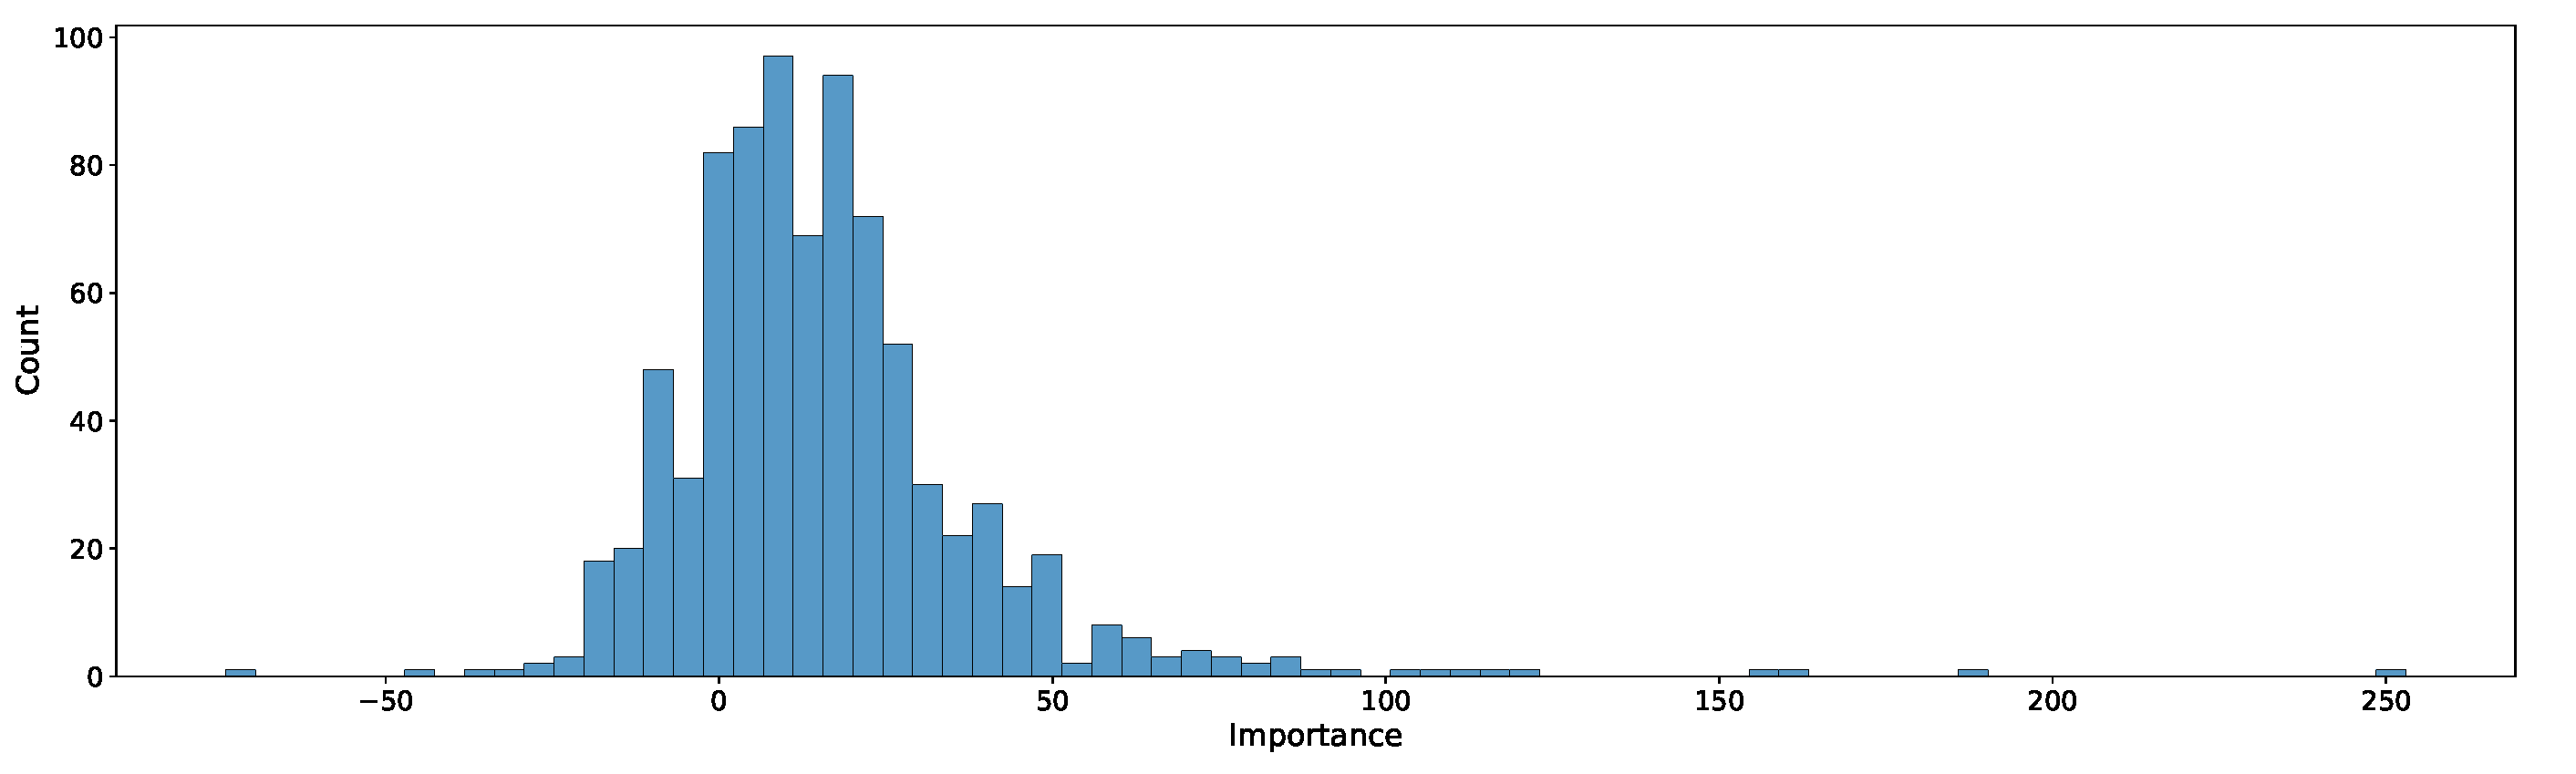
\includegraphics[width=\linewidth]{fig/abs_importance.pdf}
    \caption{A histogram of importances of $832$ features from \texttt{mixed5a}.}
    \label{fig:importance_distr}
\end{figure}

\subsection{Interpretability}
I was originally planning to use OpenAI's Microscope\footnote{\url{https://openai.com/research/microscope}}, but at the time visualizations were not accessible there. So, I decided to replicate the visualizations using Lucid. As I realized later, the appendix of~\cite{olah2017feature} also comes with visualizations for all features of InceptionV1, not only the ones shown in the paper. However, reimplementation is still useful as it can be easily adapted to other networks supported by Lucid.

I chose to measure interpretability using a visual inspection of 4 feature visualziations with a diversity term and 8 max-activation dataset examples. These visualizations were pre-computed for all features of the \texttt{mixed5a} layer. I could check that the visualizations are reasonable by comparing to visualizations from~\cite{olah2017feature}. Some examples are shown in Figure~\ref{fig:comp_viz}. We can see that the visualizations usually match diversity visualizations from the original paper (minor discrepancies are likely due to weighting the diversity versus feature maximization terms and randomness). At the same time, dataset examples do not always show matching concepts. For example, \texttt{mixed5a:4} feature is responding to flames in the original examples, but my selection fails to show this. I suspect that such occasional failures are due to the limited selection of the validation sample that I chose. I didn't use negative visualization and examples for simplicity.

The measurement metrics, detailed survey guidelines, and expected results were pre-recorded in a Google doc\footnote{\url{https://docs.google.com/document/d/1_xDxej78VRy_xRjoJ7SecTBaEWsnTHy4s7bSXkBqRNo/edit?usp=sharing}}. My metric for ``interpretability'' is derived from two equally weighted components. First, how predictable are the dataset examples given only the visualizations. Second, how coherent are the examples between each other. I also tried to measure some notion of ``polysemanticity'' in the features but in practice found that my visualizations do not allow for a clear distinction of polysemantic neurons against non-interpretable ones. To be specific, I implemented a form that shows the generated images and asks a participant several questions about what they see. First, only the four visualizations are shown. The following two questions are asked:
\textit{
\begin{enumerate}
  \item On a scale from 1 to 5, how clear are the objects on the 4 feature visualization images? If you can’t recognise any objects on the images, respond as 1:
  \item Which words or phrases are best describing objects on the feature visualization images. List 0-4 phrases through comma:
\end{enumerate}
}

After the participant fills out these questions and submits, the dataset examples are revealed and the participant has the opportunity to compare the examples against the phrases that they recorded in Q.2. The following questions become available:
\textit{
\begin{enumerate}
  \setcounter{enumi}{2}
  \item On a scale from 1 to 5, how closely do the dataset examples resemble the phrases you put in the previous question? Respond 1 if you didn’t write any phrases:
  \item On a scale from 1 to 5, how coherent are the examples (i.e. 1=they have nothing in common, 5=they all show the same concept)?
  \item On a scale from 1 to 5, do you agree that feature visualizations and dataset examples show 2 distinct concepts? 1 = ``There clearly aren’t two objects''; 5=``There clearly are two objects''
  \item On a scale from 1 to 5, do you agree that feature visualizations and dataset examples show 3 distinct concepts? 1 = ``There clearly aren’t three objects''; 5=``There clearly are three objects''
\end{enumerate}
}
The interface with an example set of visualizations is presented in Figure~\ref{fig:interface}. Text response to Q.2 is not used in evaluations, but it provides an accountability mechanism for the respondent to evaluate the correctness of their intuitions about the visualizations. 

Let $Q_i\in\{1,\cdots,5\}$ be the answer provided to the $i$-th question by the respondent. We denote $q_i=(Q_i-1) / 4$ as its normalized value. Then, my measure of interpretability is given by
\begin{equation}
  I=\frac{q_1q_3+q_4}{2}\in[0,1].
\end{equation}
Here, the intuition for the first term is as follows. The value is high if the respondent put high confidence into their prediction about the objects on the visualization, and then correctly predicted them. If one of these things did not happen, visualizations should not be considered informative. The other term is more straightforward, simply tracking the coherency of the dataset examples.

My idea was to get a few students from AGISF to take the survey and use their answers, but no one responded to my call, so, going against the practices, I filled out the survey myself. I shuffled the features in the two groups so that I would not know if a given visualization comes from a high- or median-importance feature. I thought to use Q.5 and Q.6 to measure polysemanticity, but when I started evaluating the features, I recognized that there were almost no situations where I could name several objects on the visualizations, and then all of them would appear in the dataset examples. At the same time, dataset examples alone are insufficient to distinguish polysemantic features from those without clearly encoded objects. These issues led me to abandon the attempt at measuring polysemanticity. 

\section{Results}
\begin{figure}[t]
    \centering
    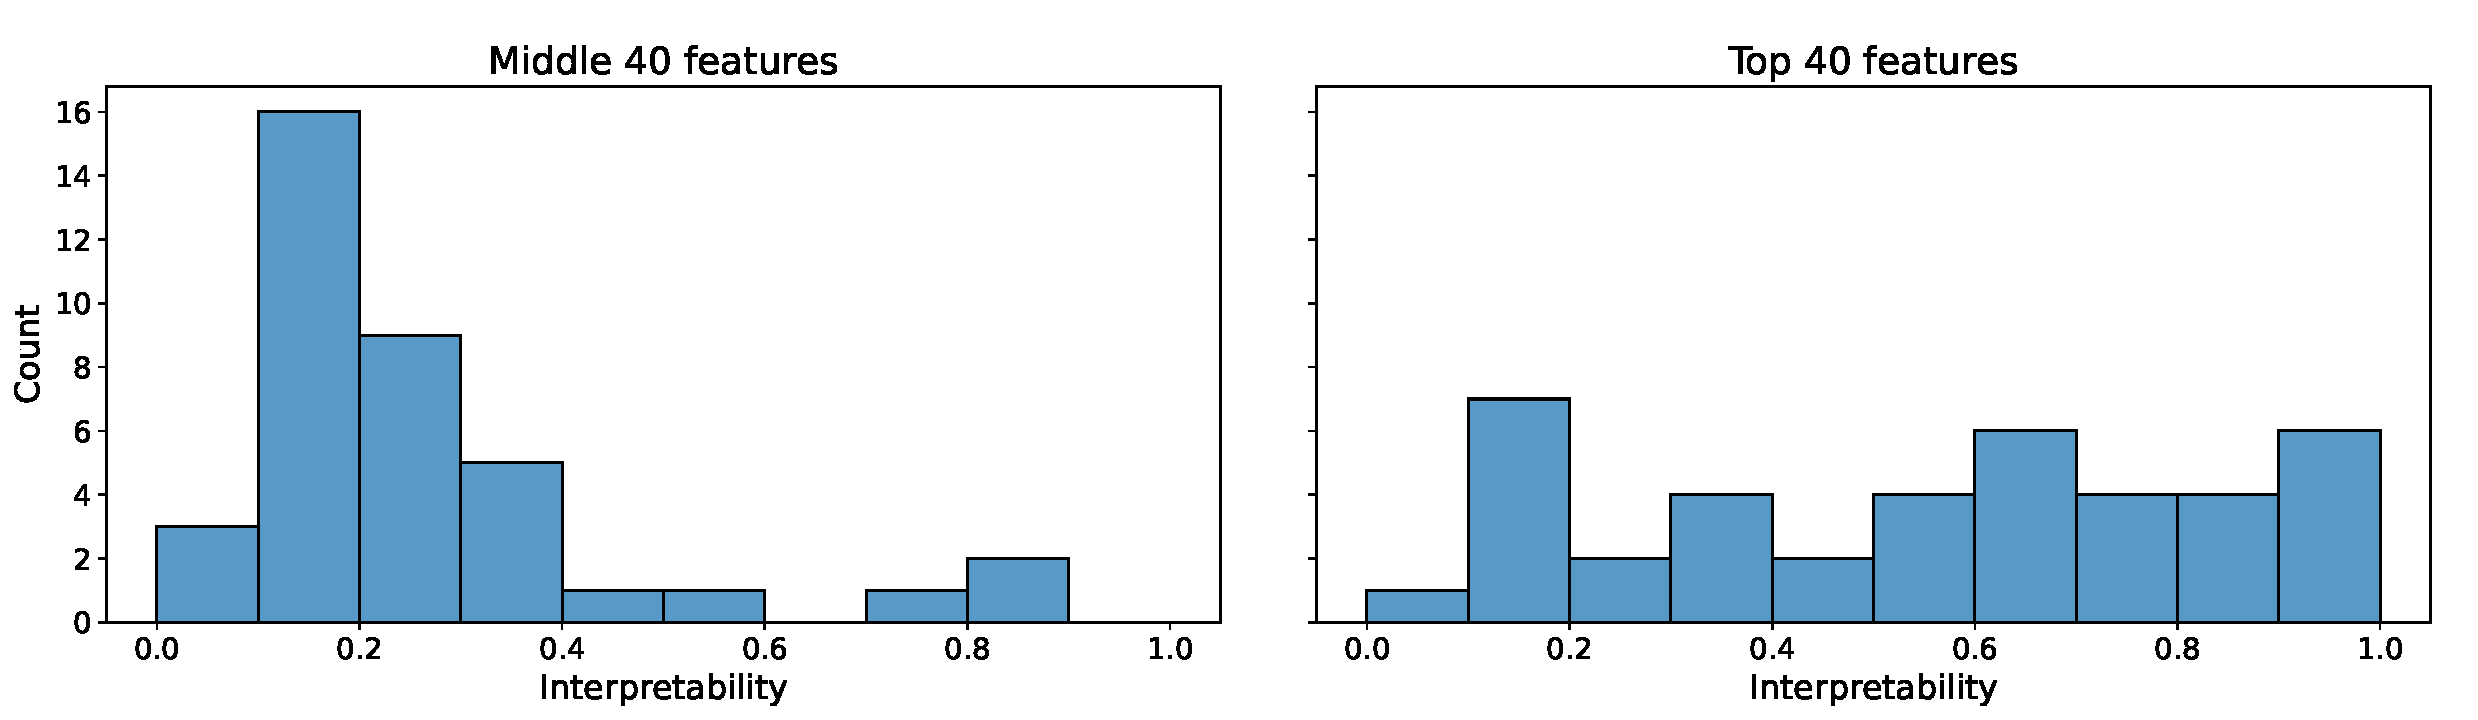
\includegraphics[width=\linewidth]{fig/groups_interp.pdf}
    \caption{Histograms of interpretability for the two groups of features.}
    \label{fig:comp}
\end{figure}
Finally, I compared the interpretability between the two groups I selected earlier based on importance. The results are presented in Figure~\ref{fig:comp}. The two groups display significant differences in values of $I$. The first one has an average of $0.24$, while the second one's average is $0.56$. In this layer of the network, the preliminary answer to the titular question of the project is \textit{yes}. We can see from the diagrams that most of the low-importance features have $I<0.5$, indicating not only that the visualizations were hard to read, but also that the dataset examples for them were incoherent, leading to low answers to Q.4. The other group, on the other hand, shows a larger variance, but all of the highest values of $I$ ended up there.

Of course, this analysis is preliminary and it is currently unclear whether it would generalize to larger models and different data modalities (e.g. text). I suspect that features reacting to single clear concepts, such as ``brown and white dog muzzle'' emerge in our situation because the number of features in the layer ($832$) is not far from the number of classes that the CNN needs to distinguish ($1000$). This allows the network to avoid polysemantic features. Another reason for the abundance of these ``clean'' interpretations of features might lie in the intermediate outputs of InceptionV1. The network was considered deep at the time of its creation, and to help with training, two extra outputs were attached to intermediate layers of the network. This might have enforced meaningful concepts to be represented early on in the layers. In modern deep networks, skip connections are used to solve the convergence issues, but they do not lead to correspondingly higher interpretability.

Analysis on a larger scale would require some automation in the measure of ``interpretability''. For example, the similarity of the dataset examples and visualizations could be measured using the Frechet Inception Distance~\cite{heusel2017gans}. Compute was also clearly a limiting factor in the project, and a larger dataset would make for better examples and importance evaluations.

This project touched on two common approaches to interpretability research. One consists of visualization of the components of a network, the other --- of causal interventions to reveal the function of the component. The fact that these two methods are connected in a way described above might indicate that the network's reasoning is more ``human-like'', and give a little extra hope to the grand project of mechanistic interpretability.

\begingroup
\raggedright
\sloppy
\bibliographystyle{abbrv}
\bibliography{report}
\endgroup


\clearpage

\begin{figure}[p]
  \centering

  \begin{subfigure}{\textwidth}
    \centering
    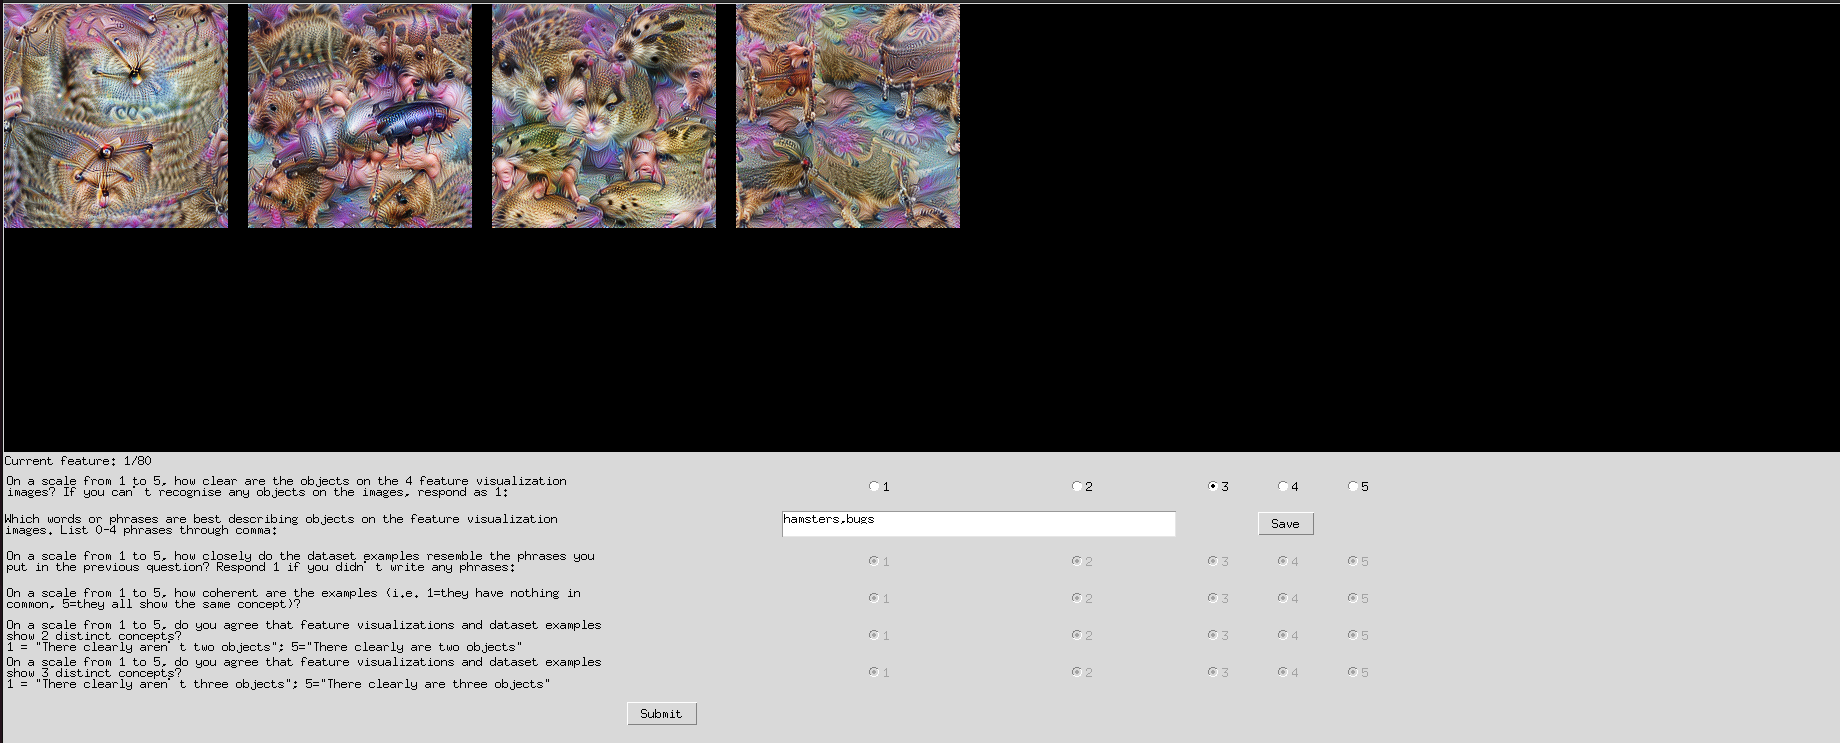
\includegraphics[width=\textwidth]{fig/interface1.png}
    \caption{Before submitting the guess about visualizations}
  \end{subfigure}
  
  \vspace{1em}

  \begin{subfigure}{\textwidth}
    \centering
    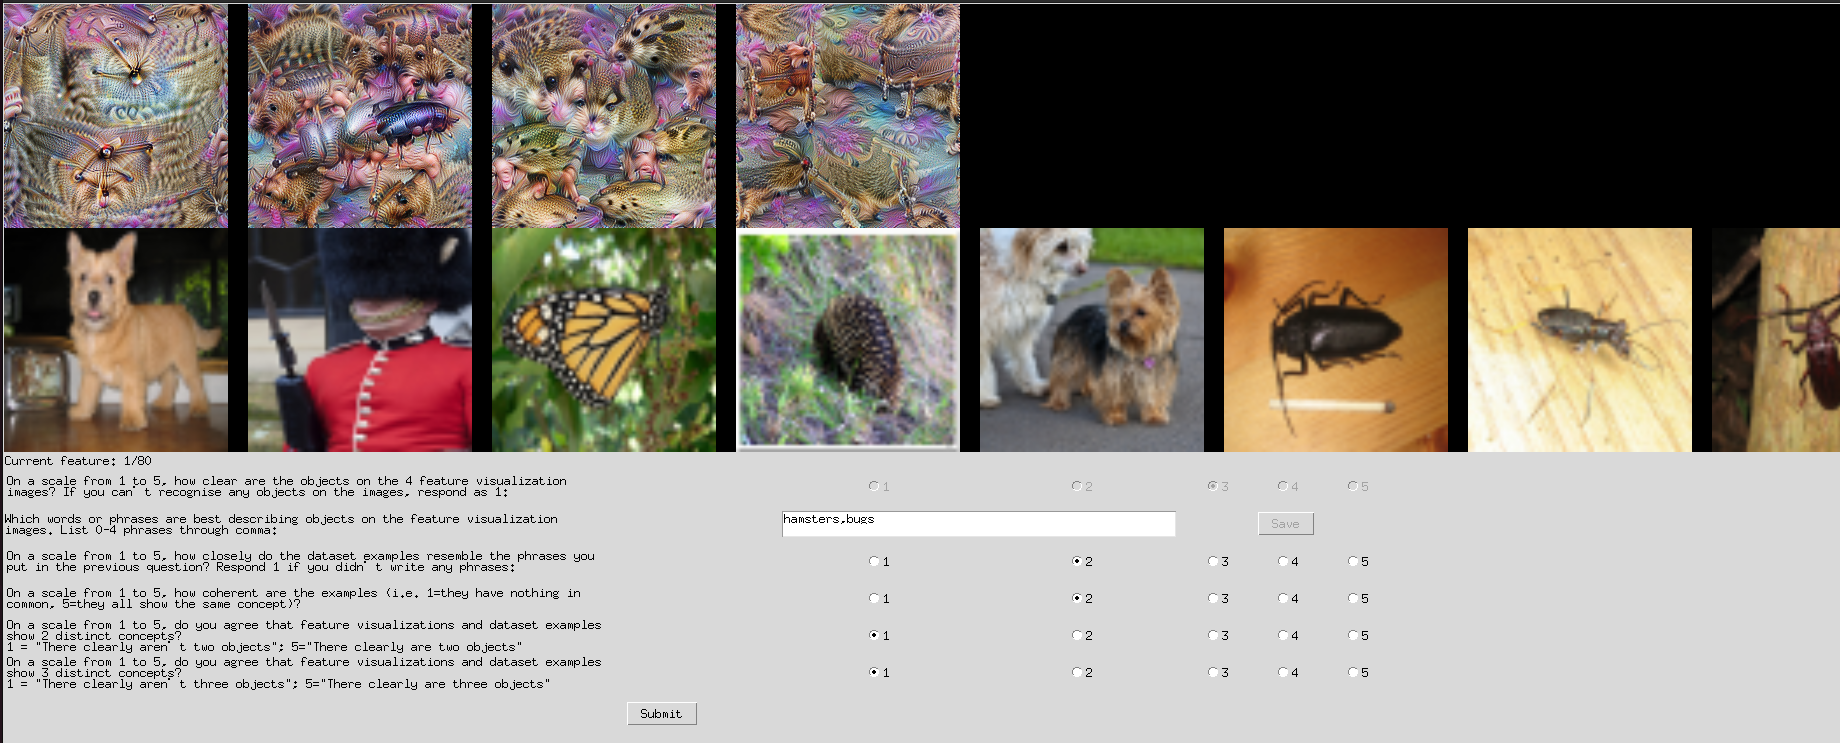
\includegraphics[width=\textwidth]{fig/interface2.png}
    \caption{After submitting the guess about visualizations}
  \end{subfigure}
  \caption{Screenshots of the interface. Questions are unintelligible here, but they correspond to the ones I provide in the text.}
  \label{fig:interface}
\end{figure}

\begin{figure}[p]
  \centering
  \vspace{-1.5em}

  \begin{subfigure}{\linewidth}
    \centering
    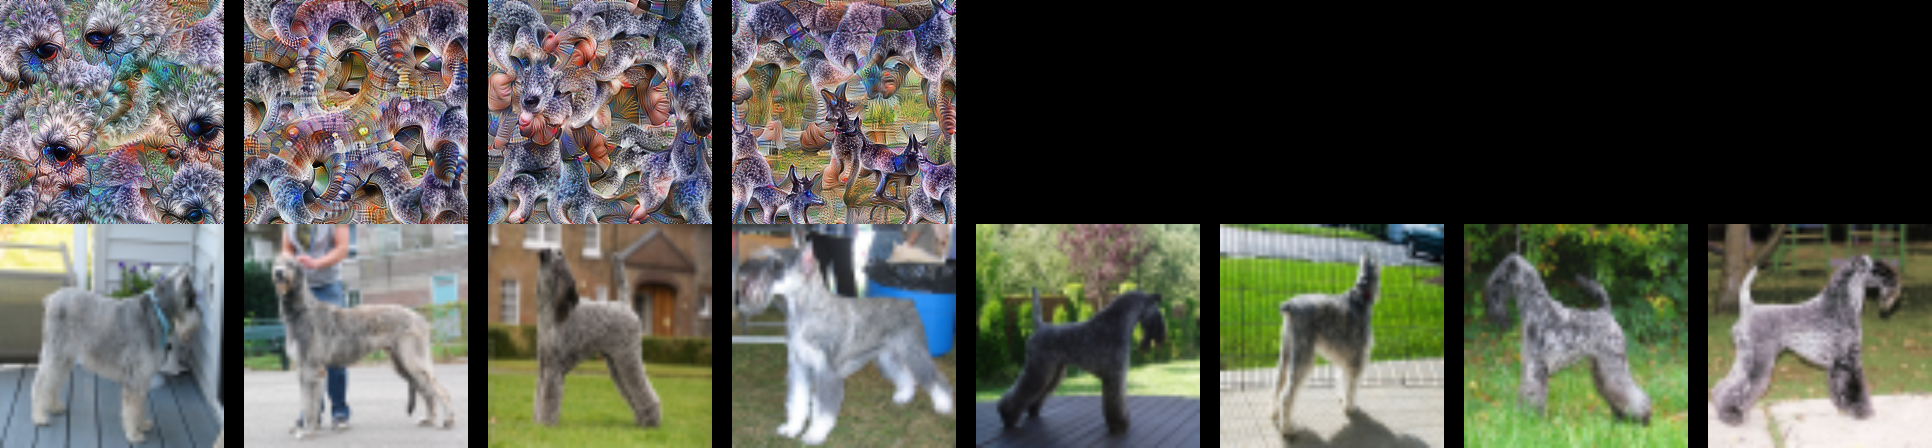
\includegraphics[width=\linewidth]{fig/mixed5a_0.png}
    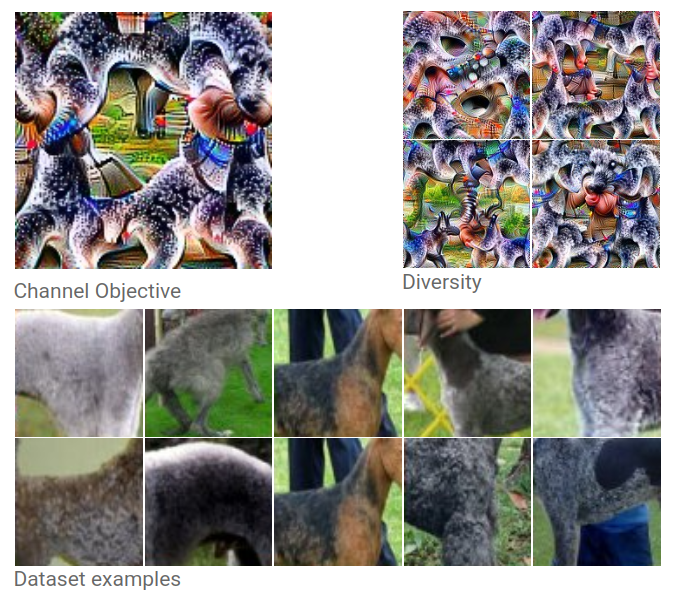
\includegraphics[width=0.4\linewidth]{fig/olah_mixed5a_0.png}
    \caption{\texttt{mixed5a:0}}
  \end{subfigure}
  
  \vspace{0.5em}

  \begin{subfigure}{\linewidth}
    \centering
    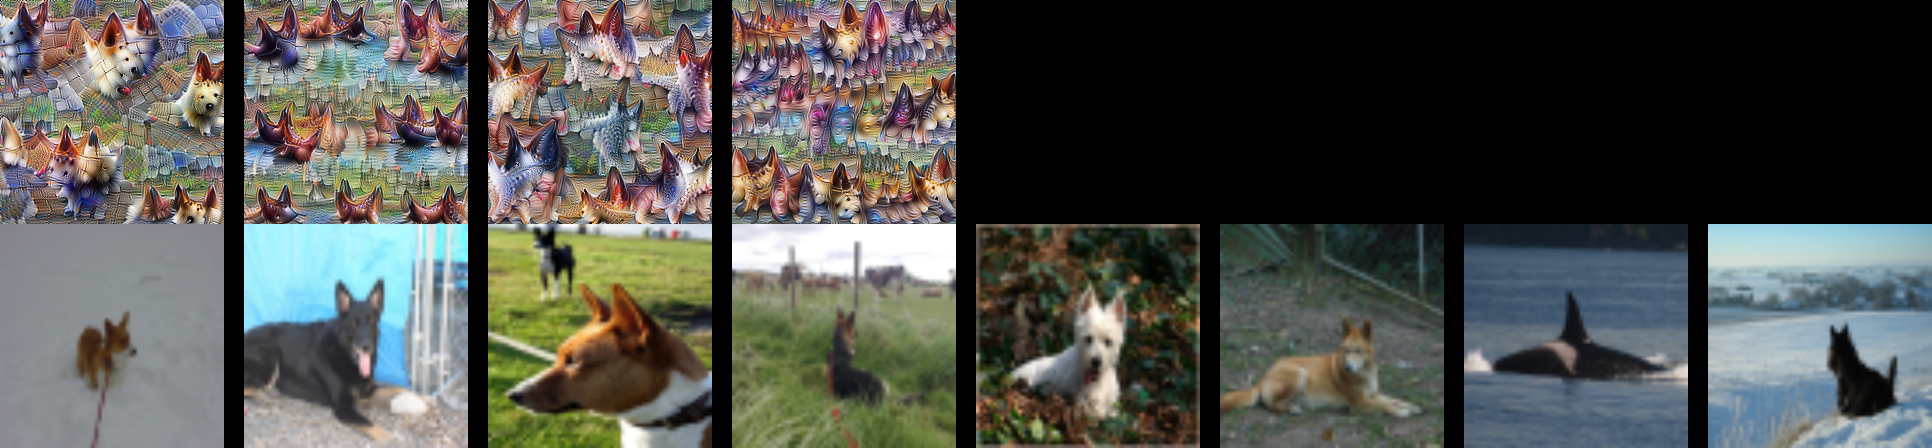
\includegraphics[width=\linewidth]{fig/mixed5a_1.png}
    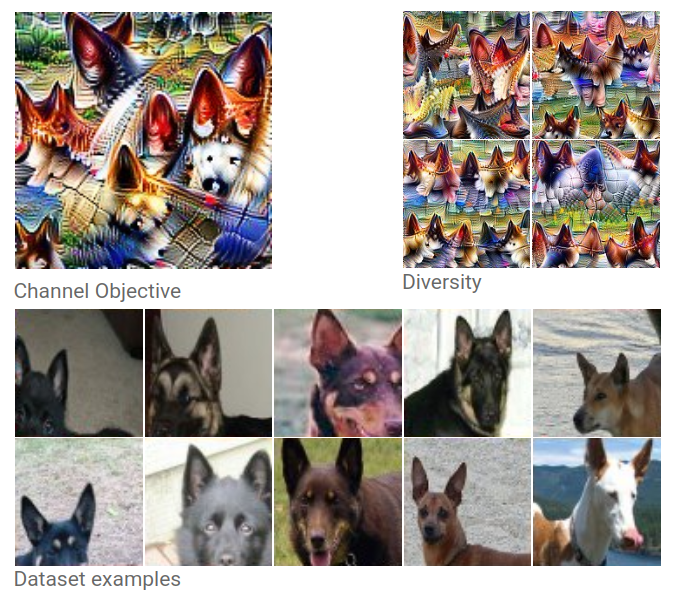
\includegraphics[width=0.5\linewidth]{fig/olah_mixed5a_1.png}
    \caption{\texttt{mixed5a:1}}
  \end{subfigure}
\end{figure}

\begin{figure}[p!]\ContinuedFloat
  \centering
  \vspace{-1.5em}

  \begin{subfigure}{\linewidth}
    \centering
    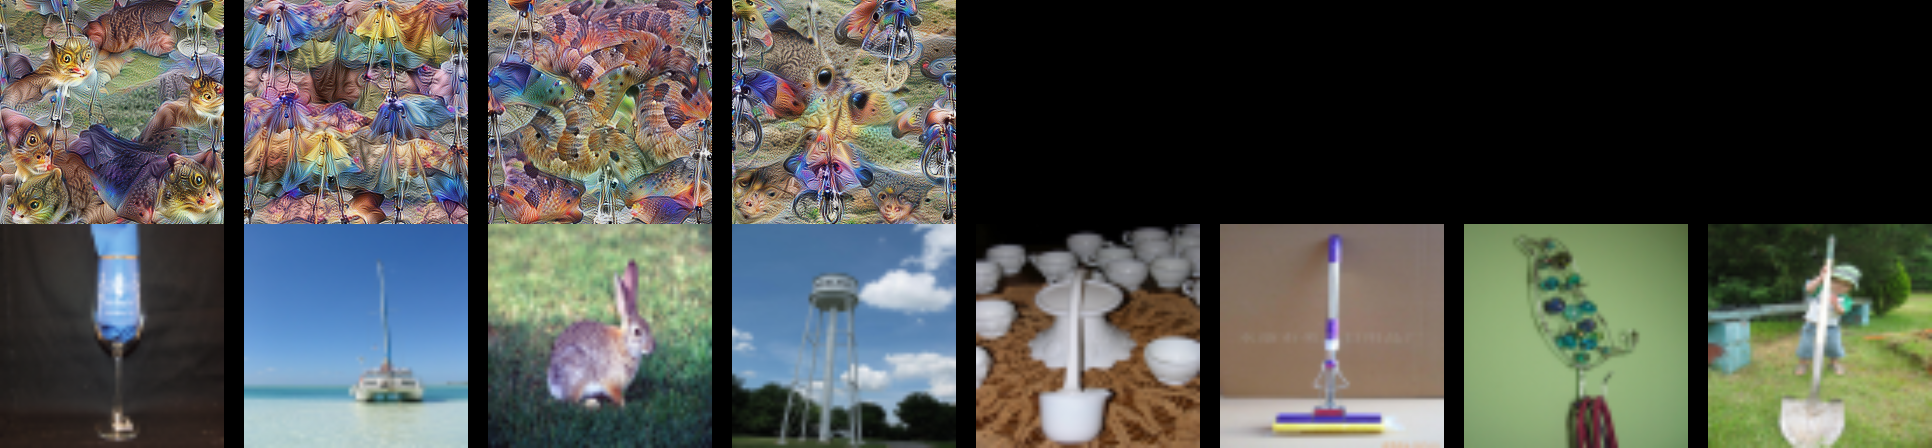
\includegraphics[width=\linewidth]{fig/mixed5a_2.png}
    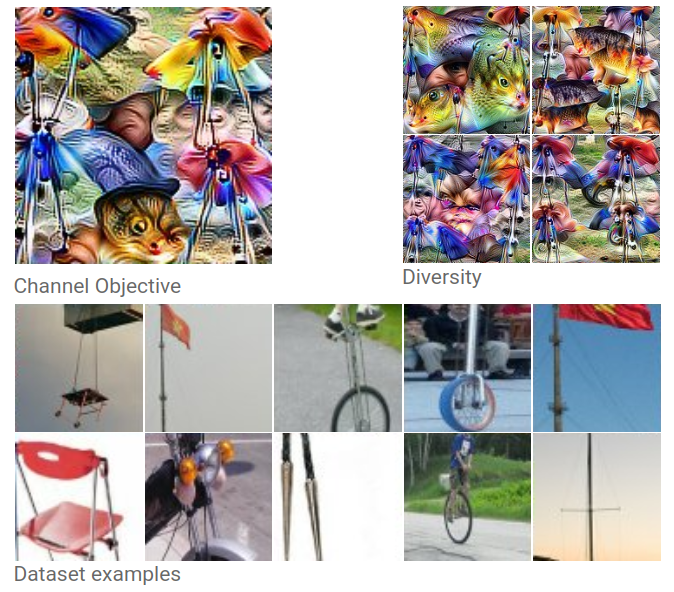
\includegraphics[width=0.4\linewidth]{fig/olah_mixed5a_2.png}
    \caption{\texttt{mixed5a:2}}
  \end{subfigure}
  
  \vspace{0.5em}

  \begin{subfigure}{\linewidth}
    \centering
    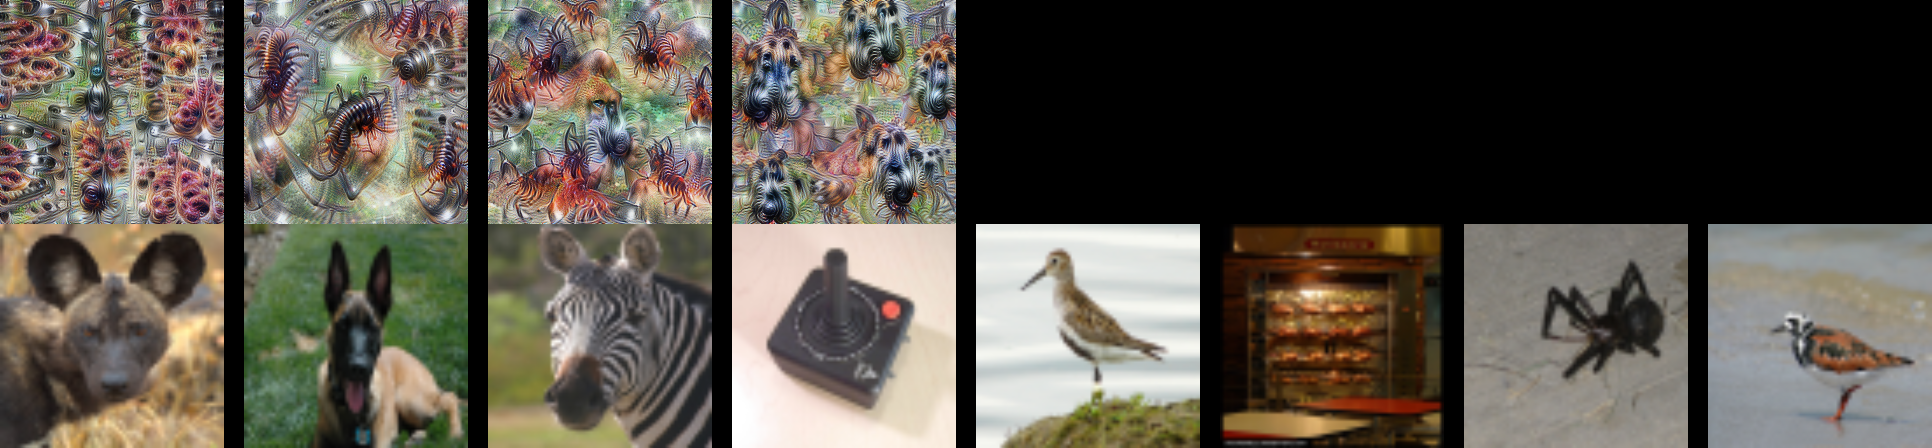
\includegraphics[width=\linewidth]{fig/mixed5a_3.png}
    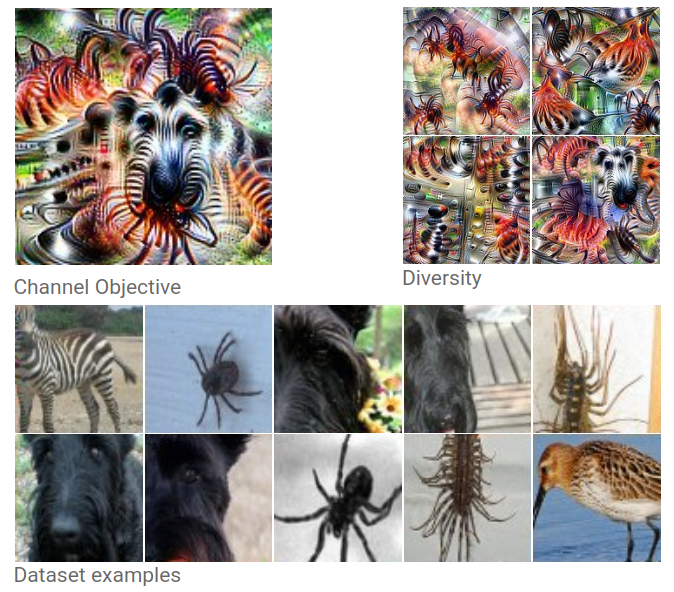
\includegraphics[width=0.5\linewidth]{fig/olah_mixed5a_3.png}
    \caption{\texttt{mixed5a:3}}
  \end{subfigure}

\end{figure}

\begin{figure}[t]\ContinuedFloat
  \centering
  \vspace{-1.5em}

  \begin{subfigure}{\linewidth}
    \centering
    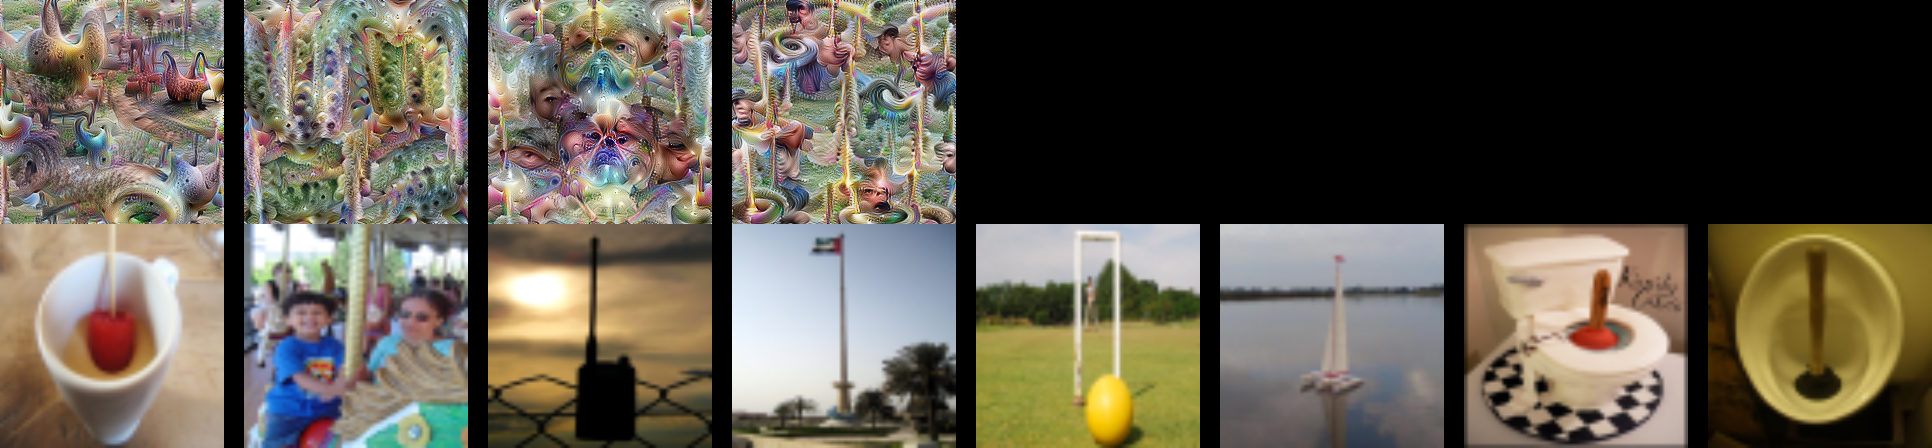
\includegraphics[width=\linewidth]{fig/mixed5a_4.png}
    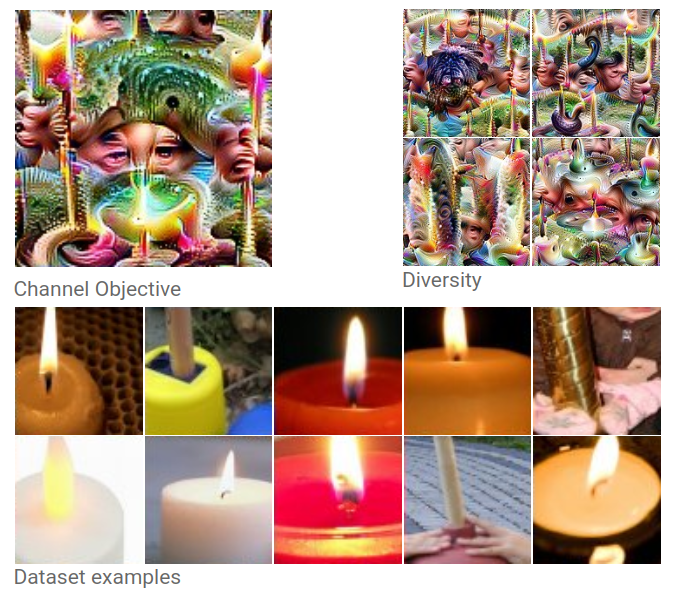
\includegraphics[width=0.4\linewidth]{fig/olah_mixed5a_4.png}
    \caption{\texttt{mixed5a:4}}
  \end{subfigure}

  \caption{5 pairs of visualizations of the first features in \texttt{mixed5a}. In each pair, the top set of images are the ones that I generated, and the bottom ones are from~\cite{olah2017feature}.}
  \label{fig:comp_viz}
\end{figure}




\end{document}


